\documentclass[12pt]{standalone}

\usepackage{tikz}


\begin{document}
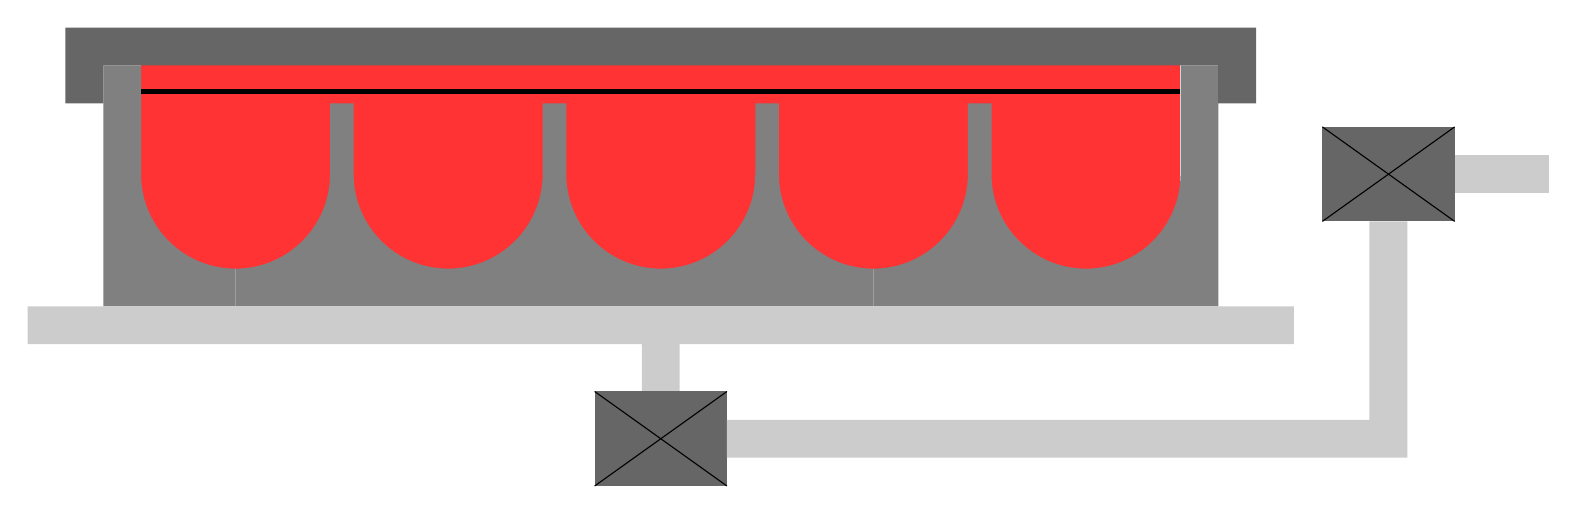
\begin{tikzpicture}[scale=.6,
elaback/.style={fill=red!30},	% Elastosil im Hintergrund
elastosil/.style={fill=red!80, opacity=1},	% flüssiges Elastosil
nichtdehnbar/.style={fill=black},	% Papierstreifen 
deckel/.style={fill=black!60},
housing/.style={fill=black!50},
rotation/.style={fill=gray!40},
motor/.style={fill=black!60}
]

%%%%%%%%%%%%%%%%%%%%%%%%%%%%%%%%%%%%%%%%5


% Defs of Basis

% Defs of Basis

\def\hy{3.5}		% Höhe y

\def\hx{2}		% Halbe Höhe x
\def\xl{.5}		% x distance luecke
\def\thick{.8}	% Halbe Dicke
	
\def\N{5}		% Anzahl Kammern



% Implicite
\pgfmathsetmacro{\hye}{\hy + \thick}		% Höhe y Elastosil level ()
\pgfmathsetmacro{\xges}{\hx+\hx+\xl}
\pgfmathsetmacro{\xgesh}{\xges/2}
\pgfmathsetmacro{\hxa}{(\xl+\thick+\thick)/3}
\pgfmathsetmacro{\X}{\xges*(\N-2)}
\pgfmathsetmacro{\Xges}{\X+2*\hx+\xges}




%%% HOUSING

\path[elastosil] (-\hx,0)--++(\Xges, 0)--++(0,\hye)--++(-\Xges, 0)--cycle;



%%%%%%%%%%%%%%% BASIS %%%%%%%%%%%%%%%%%%

\foreach \x[count=\i] in {0, \xges, ..., \X}{

\path (\x,0)coordinate(OL); 	% Koord oeben links
\def\kontur{
(OL) arc(270:360:\hx) --++(0,\hy-\hx)--++(\xl,0)--++(0,-\hy+\hx)arc(180:270:\hx)coordinate(OR)--++(0,-\thick)--++(-\xges,0)--cycle}
\path[housing] \kontur;

}

%% Enden
\path[housing](OR) arc(270:360:\hx)--++(0,\hy-\hx+\thick)--++(\thick,0)--++(0,-\hy-2*\thick)--++(-\hx-\thick,0)--cycle;
\path[housing](0,0) arc(-90:-180:\hx)--++(0,\hy-\hx+\thick)--++(-\thick,0)coordinate(HOL)--++(0,-\hy-2*\thick)--++(\hx\thick,0)--cycle;


%% nicht dehnbar

\path[nichtdehnbar] (-\hx,\hy+.2)rectangle++(\Xges,.1);

%% Deckel
\path[deckel] (HOL)--++(0,-\thick)--++(-\thick,0)--++(0,2*\thick)--++(\Xges+4*\thick,0)--++(0,-2*\thick)--++(-\thick,0)--++(0,\thick)--cycle;




%% Rotation
\pgfmathsetmacro{\brot}{\Xges+6*\thick}
\path[rotation] (-\hx+\Xges/2,-\thick)--++(-\brot/2,0)--++(0,-\thick)--++(\brot/2-\thick/2,0)--++(0,-1)coordinate(S)--++(\thick,0)--++(0,1)--++(\brot/2-\thick/2,0)--++(0,\thick)--cycle;

\path[motor] (S)++(-1,0)coordinate(X)rectangle++(2+\thick,-2);
\draw (X)--++(2+\thick,-2) ++(0,2)--++(-2-\thick,-2);

\path[rotation] (X)++(2+\thick,-1)--++(0,-\thick/2)--++(\brot/2+1,0)--++(0,5)coordinate(S)--++(-\thick,0)--++(0,-5+\thick)--++(-\brot/2-1+\thick,0)--cycle;

\path[motor] (S)++(1,0)coordinate(X)rectangle++(-2-\thick,2);
\draw (X)--++(-2-\thick,2) ++(0,-2)--++(2+\thick,2)++(0,-1)coordinate(S);

\path[rotation] (S)++(0,-\thick/2)rectangle++(2,\thick);

\end{tikzpicture}
\end{document}